%%% Local Variables:
%%% mode: latex
%%% TeX-master: t
%%% End:
% --------------------------------------------------------------
% This is all preamble stuff that you don't have to worry about.
% Head down to where it says "Start here"
% --------------------------------------------------------------

\documentclass[12pt]{article}

\usepackage[margin=1in]{geometry}
\usepackage{amsmath,amsthm,amssymb}
\usepackage{graphicx}

\newcommand{\N}{\mathbb{N}}
\newcommand{\Z}{\mathbb{Z}}

\newenvironment{theorem}[2][Theorem]{\begin{trivlist}
\item[\hskip \labelsep {\bfseries #1}\hskip \labelsep {\bfseries #2.}]}{\end{trivlist}}
\newenvironment{lemma}[2][Lemma]{\begin{trivlist}
\item[\hskip \labelsep {\bfseries #1}\hskip \labelsep {\bfseries #2.}]}{\end{trivlist}}
\newenvironment{exercise}[2][Exercise]{\begin{trivlist}
\item[\hskip \labelsep {\bfseries #1}\hskip \labelsep {\bfseries #2.}]}{\end{trivlist}}
\newenvironment{reflection}[2][Reflection]{\begin{trivlist}
\item[\hskip \labelsep {\bfseries #1}\hskip \labelsep {\bfseries #2.}]}{\end{trivlist}}
\newenvironment{proposition}[2][Proposition]{\begin{trivlist}
\item[\hskip \labelsep {\bfseries #1}\hskip \labelsep {\bfseries #2.}]}{\end{trivlist}}
\newenvironment{corollary}[2][Corollary]{\begin{trivlist}
\item[\hskip \labelsep {\bfseries #1}\hskip \labelsep {\bfseries #2.}]}{\end{trivlist}}

\begin{document}

% --------------------------------------------------------------
%                         Start here
% --------------------------------------------------------------

\newcommand{\ijk}{(i, j, k)}

\title{CS5214 Design of Optimizing Compilers }%replace X with the appropriate number
\author{Professor Weng-Fai Wong\\ %replace with your name
Assignment One} %if necessary, replace with your course title

\maketitle

\abstract{
This is my solutions for assignment three problem set.
This is the answer presented by Pan An. My student number is
A0134556A.
}
% --------------------------------------------------------------
%     You don't have to mess with anything below this line.
% --------------------------------------------------------------





\section{Loop Analysis}
The flow dependency of the given loop psudo-code concerns only
variable list $X$. Here we denote the only value assignment in the
loop as
$$X[\vec{f}\ijk] = X[\vec{g}\ijk]$$

\subsection{Formulation}
So in this case if we need to take care of the formulation there are
three equations that we need to satisfy:
\begin{equation}
\begin{aligned}
3j_s + k_s &= & 2i_t +4k_t\\
i_s + 2j_s + k_s &= & 5j_t + 7k_t\\
2j_s + 3k_s &= & 3i_t + 5j_t\\
\end{aligned}
\end{equation}

And $i, j, k$ subject to:

\begin{equation}
\begin{aligned}
0 < & ~i_s, i_t< 11\\
0 < & ~j_s, j_t< 51\\
0 < & ~k_s, k_t< 21
\end{aligned}
\end{equation}

%
%
%
So here I'm gonna go with formulating the problem with distance
vector.
The problem defined can be expressed in matrix form: $$\pmb{V\cdot A < b }$$
 where:
\begin{equation}
%\left[ \begin{array}{c} x_s \\ x_t \end{array} \right]
%= \begin{bmatrix} A & B \\ C & D \end{bmatrix} \times
%\left[ \begin{array}{c} y_s \\ y_t \end{array} \right]
 \pmb{V} =\begin{bmatrix}
 0 & 1  & 0  \\
 3 & 2  & 2  \\
 1 & 1 & 3 \\
-2 & 0 & -3 \\
0 & -5 & -5 \\
-4 & -7 & 0 \\

 \end{bmatrix}
\end{equation}
Which has to satisfy:

\begin{equation}
  [i_s, j_s, k_s, i_t, j_t, k_t] \begin{bmatrix}
 0 & 1  & 0  \\
 3 & 2  & 2  \\
 1 & 1 & 3 \\
-2 & 0 & -3 \\
0 & -5 & -5 \\
-4 & -7 & 0 \\

 \end{bmatrix}
= [0, 0, 0]
\end{equation}


And after Echelon Reduction we have:
\begin{equation}
  \pmb{E} = \begin{Bmatrix}
    1 & 0 & 0 \\
0 & 1 & 0 \\
0 & 0 & 1 \\
0 & 0 & 0 \\
0 & 0 & 0 \\
0 & 0 & 0 \\
  \end{Bmatrix}
~~and~~ \pmb{U}
=
\begin{bmatrix}
  -\frac{4}{7} & \frac{3}{7} & -\frac{2}{7}  & 0 & 0  & 0 \\
 1 & 0 &  0 & 0 &  0 & 0 \\
 -\frac{1}{7} & -\frac{1}{7} & \frac{3}{7} & 0 & 0 & 0 \\
-\frac{17}{21}& \frac{1}{3} & 0 & \frac{12}{7}  & 0 & 0 \\
\frac{30}{7} & -\frac{5}{7} & \frac{15}{7} & 0 & 1 & 0 \\
\frac{59}{21}& \frac{12}{7} & -\frac{8}{7} & 0 & 0 & 1 \\
\end{bmatrix}
\end{equation}

And in order to do finish the back substitution have to let
$\pmb{t\cdot E = 0}$. Next we will be conducting Fourier-Motzkin
Elimination.

\subsection{Fourier-Motzkin Elimination}
Okay so when I finish the last chapter I suddenly relize that what I
was required to do is to give the process of Fourier-Motzkin
Elimination. Anyway I just leave the stuff there.

And according the the previous result. $\pmb{t}$ must satisfy:
\begin{equation}
  \begin{aligned}
    0 <& -\frac{17}{21}t_4 + \frac{30}{7}t_5 + \frac{59}{21}t_6 &< 11 \\
    0 <& ~~~~~~~\frac{1}{3}t_4 - \frac{5}{7} + \frac{12}{7} &< 51 \\
0 <&~~~~~~~~~\frac{15}{7}t_5 - \frac{8}{7}  &< 21 \\
0 <& ~~~~~~~~~~~~~\frac{12}{7}t_4   &<  11 \\
0 <& ~~~~~~~~~~~~~~~t_5 &< 51 \\
0 <& ~~~~~~~~~~~~~~~ t_6 &< 21 \\
  \end{aligned}
\end{equation}

There is actually solution to this one.





\subsection{Omega Test}



\section{Loop Tiling}

Considering that in this problem X and Y has exactly the same size. There is no need to take into consideration
the utilization of loop interchange.

Anyway, the principle of loop tiling is to load  into the
the cache as less times  as possible. Also in this case only 8 digits
are allowed in each cache line. The sudo code for tiling is shown as
below:

\begin{verbatim}
for (int i = 0; i < n; i += blocksize) {
    for (int j = 0; j < n; j += blocksize) {
        // the block below will then be sent
        for (int k = i; k < i + blocksize; ++k) {
            for (int l = j; l < j + blocksize; ++l) {
                X[k, l] = Y[l, k];
            }
        }
    }
}
\end{verbatim}

The available cache integer storage is 8 digits. So here the block
size should be 2, this way, every $2\times 2$ block of both $x$ and
$y$ will be loaded to the cache and processed.

The loop will be excuted as the following graph shows:

\begin{figure}[!ht]
  \centering
  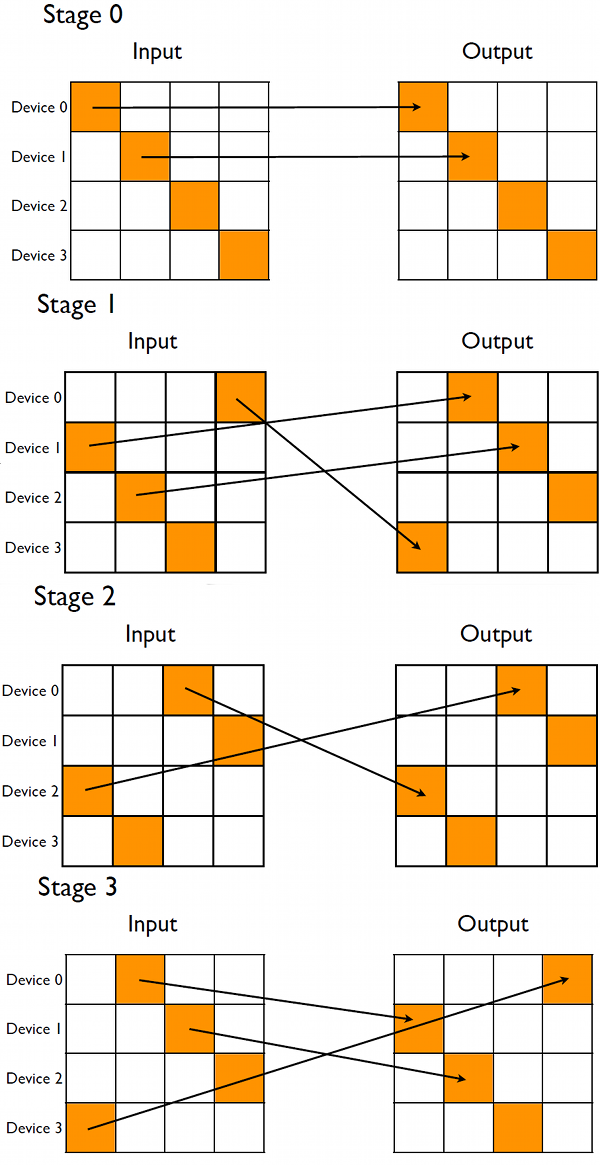
\includegraphics[scale=0.2]{img/tilling.png}
  \caption{Simple Graph of Tiling.}
  \label{fig:n}
\end{figure}

In \ref{fig:n} the input means the matrix of y and the output is the
matrix  of x. Each block represents a $2\times 2$ block.

The cache hit, before the tiling, should be 50\%. Considering that
only 8 digits were in the cache. And after the tiling it should be
100\%, since it only loads the piece of matrix that is needed to do
the transpose.






\end{document}

%%% Local Variables:
%%% mode: latex
%%% TeX-master: t
%%% End:
